\documentclass[a4paper,11pt]{article}
\usepackage{multicol}
%\usepackage{multitoc}
%\usepackage{german}
%\usepackage{bibgerm}
\usepackage{amsmath}
\usepackage{amsfonts}
\usepackage{xspace}
\usepackage[body={148mm,240mm,nohead}]{geometry}
\usepackage[ansinew]{inputenc}
\usepackage{listings}
\usepackage{relsize}
\usepackage{tikz}
\usepackage{hyperref}
\lstset{language=C++, basicstyle=\ttfamily,
  stringstyle=\ttfamily, commentstyle=\it, extendedchars=true}

\usepgflibrary{arrows}

\newcommand{\dune}{\textsc{Dune}\xspace}
\newcommand{\modulename}[1]{\texttt{#1}\xspace}
\DeclareMathOperator\sgn{sgn}

\title{The dune-localfunctions module}

\author{The \dune Team}

\date{\today}

\begin{document}

\maketitle

\begin{abstract}
This document describes the \modulename{dune-localfunctions} module.
The module provides a C++ interface for shape functions needed in
finite element methods.  A growing list of implementations of this
interface is included. \modulename{dune-localfunctions}
is part of the Distributed and Unified Numerics Environment (\dune) which is
available from the site \url{http://www.dune-project.org/}.
\end{abstract}

\begin{multicols}{2}
{\small\tableofcontents}
\end{multicols}

\section{Introduction}

A feature common to all implementations of finite element methods are the
shape functions.  In the easier cases, these are polynomial functions
defined on a reference element and associated to some face of the reference
element.  The more complicated non-affine finite elements generalize this
by defining the shape functions directly on an element in the grid.

Implementations of shape functions are contained in all finite element codes,
but in most cases their implementation is so intertwined with the rest of
the code as to make their reuse in other situations impossible.
For the easier shape functions this may not matter much, as they are
fairly easy to implement.  Still, errors can occur and bugs in shape function
implementations can be difficult to detect and track down.
More exotic shape function implementations can get fairly involved
and require meticulous care to be done right.  For these reasons it is
very desirable to provide shape functions in a separate, reusable library.
This is what the \modulename{dune-localfunctions} module tries to do.


Following the UNIX philosophy of having each program doing only one thing,
but doing that thing well, the \modulename{dune-localfunctions} module
provides only local and global finite elements.  There are two sides to this.
\begin{enumerate}
 \item \modulename{dune-localfunction} prescribes an {\em interface} to shape functions.
  This interface
  should be general enough to encompass the needs of virtually all implementors
  of finite element codes.
 \item The module contains {\em implementations} of this interface.  The set
  of implementations contains common elements like the Lagrange elements and
  exotic ones as well.  We aim to collect contributions from outside sources
  and, in time, to be able to provide a shape function library that is virtually
  complete.
\end{enumerate}

\subsection{Static vs.\ Dynamic Interfaces}

From a textbook C++ perspective, an interface to finite element shape functions
can be described naturally using dynamical polymorphism.  An abstract base
class would describe all methods expected from a shape function implementation,
and actual implementations would derive from the base class.  Users of shape functions,
such as finite element assemblers, would receive shape function implementations
through pointers to the abstract base class.

However, the run-time overhead of virtual function calls is considered prohibitive
by some users.  We measured a slowdown of around 7\% when assembling a Laplace
stiffness matrix on a two-dimensional structured grid.  This can be relevant,
for example, in an explicit time-stepping method where a large percentage of
the overall time is spent assembling matrices.

We have therefore opted for a different way.  In \modulename{dune-localfunctions},
the implementation classes are {\em not} organized in a hierarchy.  Adherence
to a certain interface is enforced only implicitly, by a test suite.  Finite
element assemblers have to have the C++ type of the shape function implementation
as a template parameter, and can then call the object's methods directly.
The static interface is described in Section~\ref{sec:static_interface}.

Of course such a scheme makes it impossible to select shape function sets at run-time.
For example, $p$-adaptive methods, and methods on grids with more than a single
element type are precluded.  Therefore, \modulename{dune-localfunctions} offers
a second way to access its shape functions.  There is a set of {\em wrapper classes},
which are organized in a hierarchy using dynamical polymorphism.  These
wrapper classes are statically parametrized with a static implementation class
and forward the function calls to this implementation.  Details of this
{\em dynamic interface} are given in Section~\ref{sec:dynamic_interface}.

\subsection{Dependencies on other Modules}

When designing the \modulename{dune-localfunctions} module we have deliberately
tried to keep dependencies on other \dune modules to a minimum.  Ideally,
people should be able to use the shape functions from \dune without having
to use anything else from \dune.  The only exception here is \modulename{dune-common},
which all \dune modules depend on.

In addition to \modulename{dune-common}, \modulename{dune-localfunctions} currently
depends only on \modulename{dune-grid}.  This dependence is somewhat unfortunate,
and it has been hotly debated.  We would like users to be able to use \dune grids
without shapefunctions from \modulename{dune-localfunctions} and the shapefunctions
from \modulename{dune-localfunctions} without the grids from \modulename{dune-grid}.
While the former is easy, \modulename{dune-localfunctions} currently needs a few
features from \modulename{dune-grid} to work.  These are in particular a few
quadrature rules and some of the infrastructure for constructing reference elements.
More seriously, \modulename{dune-localfunctions} provides some {\em global} finite
elements (also known as {\em non-affine families} of finite elements).  These
have to have some information about the geometry of the grid.

In the future the necessary things from \modulename{dune-grid} may be split off
into a separate module \modulename{dune-geometry} (or similar).  The dependence of
\modulename{dune-localfunctions} on \modulename{dune-grid} can then be replaced
by the weaker dependency on the new module.


\section{The \lstinline!LocalFiniteElement! Interface}
\label{sec:static_interface}
The interface of a \lstinline!LocalFiniteElement! is designed to provide the user
with all the functionality needed for the implementation of finite element methods.
The functionality consists of three subtasks.  These are handled by separate classes
which can be obtained from the \lstinline!LocalFiniteElement! class.
\begin{enumerate}
\item The assembly of the local stiffness matrices usually requires the evaluation
   of the shape functions and/or their derivatives of a certain order $k$ on the
   reference element.  These features are collected in a \lstinline!LocalBasis! class. 
\item For the correct distribution of the local matrices to the global stiffness matrix
   one needs to associate the individual shape functions to subentities (i.e., vertices,
   faces, elements,\dots) of the reference element.  This information is provided
   by a \lstinline!LocalCoefficients! class.  An \lstinline!IndexSet! class can
   then be used to obtain global indices for each shape function.
\item Finally one needs to interpolate given functions by the shape functions.
   This functionality is provided by the \lstinline!LocalInterpolation! class.
\end{enumerate}
Motivated by these points the  interface of a \lstinline!LocalFiniteElement! is given by:
\begin{lstlisting}
class LocalFiniteElementInterface
{
   // export traits 
   typedef LocalFiniteElementTraits<LocalBasisImpl,
 	LocalCoefficientsImpl, LocalInterpolationImpl> Traits;

   // access to the local basis implementation
   const Traits::LocalBasisType& localBasis() const;

   // access to the local coefficient implementation
   const Traits::LocalCoefficientsType& localCoefficients() const;

   // access to the local interpolation implementation
   const Traits::LocalInterpolationType& localInterpolation() const;
   
   // geometry type the local basis lives on
   GeometryType type() const;
};
\end{lstlisting}
The \lstinline!LocalFiniteElementTraits! class is a simple traits helper struct that can be used for the export of the class traits.

Each local finite element has to provide an implementation of the three classes that are described in the next sections.

\subsection{The \lstinline!LocalBasis! Classes}
The \lstinline!LocalBasis! class represents the set of shape functions:
\begin{lstlisting}
class LocalBasisInterface
{
   // export type traits for shape function signature
   typedef LocalBasisTraits<DF,n,D,RF,m,R,J> Traits;

   //number of shape functions
   unsigned int size () const;

   // evaluate all shape functions at a given position 
   inline void 
   evaluateFunction(const typename Traits::DomainType& in,    
             std::vector<typename Traits::RangeType>& out) const;

   // evaluate Jacobian of all shape functions at a given position
   inline void 
   evaluateJacobian(const typename Traits::DomainType& in,  
             std::vector<typename Traits::JacobianType>& out) const; 

   // evaluate general derivative of k-th order of all shape functions
   template<unsigned int k>
   inline void 
   evaluate (const typename Dune::array<int,k>& directions,  
             const typename Traits::DomainType& in,    
             std::vector<typename Traits::RangeType>& out) const;

   // polynomial order of the shape functions
   unsigned int order () const;
};
\end{lstlisting}
The \texttt{LocalBasisTraits} class is a traits helper class which holds information on how the signature
of the shape functions is represented in C++ types. A description of the template parameter above can
be found in the doxygen documentation of the traits class. 

\subsection{The \lstinline!LocalCoefficients! Classes}
To describe the position of the degrees of freedom (shape functions) of a \lstinline!LocalFiniteElement!
it is assumed that each degree of freedom can be attached to a subentity of the underlying reference element.
For every degree of freedom we thus have
\begin{enumerate}
\item the local number of the associated subentity \texttt{s},
\item the codimension of the subentity \texttt{c},
\item the index in the set of all shape functions associated to this subentity \texttt{t}.
\end{enumerate} 
These informations are stored in the \lstinline!LocalKey! class, which allows
access to the entries by the methods \lstinline!subentity()!, \lstinline!codim()!, and \lstinline!index()!.
For the correct local numbering of the subentities see the documentation of the \lstinline!GenericReferenceElements!
at \url{http://dune-project.org}.

The \lstinline!LocalCoefficient! class now associates the indices of the shape function with
their corresponding \lstinline!LocalKey!s.
\begin{lstlisting}
class LocalCoefficientsInterface
{
   // number of coefficients
   std::size_t size () const;

   // get i-th index
   const LocalKey& localKey (std::size_t i) const;

};
\end{lstlisting}

\subsection{The \lstinline!LocalInterpolation! Classes}
\begin{lstlisting}
class LocalInterpolationInterface 
{
// export local basis traits
LocalBasisInterface::Traits Traits;

// local interpolation of a function
template<typename F, typename C>
void interpolate (const F& f, std::vector<C>& out) const;
};
\end{lstlisting}
The \lstinline!LocalInterpolation! class provides a method to interpolate a given function
and that returns a coefficient vector for the shape functions. The function  class
to interpolate must provide a method
\lstinline!evaluate(const Traits::DomainType& x, Traits::RangeType& y)!,
which is used to evaluate the function on the reference element of the corresponding geometry type.

\section{The Dynamic Interface}
\label{sec:dynamic_interface}

In some situations one doesn't know at compile time which shape function set is needed.
This happens for example when grids with several element types are involved or $p$-adaptive
methods are used. For this case \modulename{dune-localfunctions} provides a way to select
shape functions at run-time.   As already described above the implementations
of \lstinline!LocalFiniteElement!s are not organized in a hierarchy. Thus,
to use dynamic polymorphism we first need a virtual interface and to avoid 
copying the code we also need a way to re-arrange the existing shape function implementations
in a hierarchy. This re-arrangement is done with the help of virtual wrapper classes
which take a static implementation as template parameter and forward the dynamic function
calls to that implementation. 

\subsection{The Virtual Interface}
From Section \ref{sec:static_interface} we know that in \modulename{dune-localfunctions}
a \lstinline!LocalFiniteElement! consists of a \lstinline!LocalBasis!,
\lstinline!LocalCoefficients!, and \lstinline!LocalInterpolation! class.  So if we want
to design a virtual interface for a \lstinline!LocalFiniteElement! we first need
to define abstract base classes for these three classes.

\paragraph{\lstinline!LocalBasisVirtualInterface!}
The \lstinline!LocalBasisVirtualInterface! is organized in a recursive hierarchy of the form
\begin{lstlisting}
template<class T>
class LocalBasisVirtualInterface :
 public virtual LocalBasisVirtualInterface<LowerOrderLocalBasisTraits<T> >
{
 typedef LocalBasisVirtualInterface<LowerOrderLocalBasisTraits<T> > Base;
public:   
 typedef T Traits;
 using Base::size;
 using Base::order;
 using Base::evaluateFunction;
 using Base::evaluateJacobian;
  
 virtual void evaluate (
  const typename Dune::template array<int,Traits::diffOrder>& directions,
  const typename Traits::DomainType& in,
  std::vector<typename Traits::RangeType>& out) const = 0;
  
};
\end{lstlisting}
The \lstinline!LowerOrderLocalBasisTraits! defines a \lstinline!LocalBasisTraits! class
(see \ref{sec:static_interface}) with \lstinline!diffOrder! reduced by one
(the \lstinline!diffOrder! of a \lstinline!LocalBasis! specifies the maximal order of
implemented partial derivatives). 
This hierarchy is needed because each \lstinline!LocalBasis! implementation is assumed
to have a template method
\lstinline!evaluate<unsigned int k>(Dune::array<int,k> directions,...)!  where 
\lstinline!k! denotes the total order of mixed partial derivatives to be computed. 
In the dynamic case this method has to be replaced by non-template methods
\lstinline!evaluate(Dune::array<int,fixedOrder> directions,...)! and the hierarchy
just makes sure that there will be a corresponding method for all 
$0 \leq $\lstinline!fixedOrder! $\leq$ \lstinline!diffOrder!. Finally a template specialization
for the case \lstinline{diffOrder = 0} provides all pure virtual methods that belong
to a \lstinline{LocalBasis}.
In the online class documentation of \modulename{dune-localfunctions} you will find another
interface class called \lstinline{LocalBasisVirtualInterfaceBase}:  
The virtual interface additionally provides a non-virtual template method
\lstinline{evaluate} which internally calls the non-template \lstinline!evaluate! method.
For name resolution reasons this method can thus not be defined in the same class,
so there is a second base class, the \lstinline{LocalBasisVirtualInterfaceBase},
which lies between two \lstinline!diffOrder! - levels and that contains this
additional method. Note that in applications you should always use the standard
\lstinline!LocalBasisVirtualInterface! class.

\paragraph{\lstinline!LocalCoefficientsVirtualInterface!}
The \lstinline!LocalCoefficientsVirtualInterface! is just the straightforward base class
containing the pure virtual methods:
\begin{lstlisting}
class LocalCoefficientsVirtualInterface
{
public:

  virtual ~LocalCoefficientsVirtualInterface() {}

  //! number of coefficients
  virtual std::size_t size () const = 0;

  //! get i'th index
  const virtual LocalKey& localKey (std::size_t i) const = 0;
};
\end{lstlisting}

\paragraph{\lstinline!LocalInterpolationVirtualInterface!}
For the \lstinline!LocalInterpolationVirtualInterface! we need a similar construction
as for the \lstinline!LocalBasisVirtualInterface!. Again we have a template method in the static 
\lstinline!LocalInterpolation! interface, namely  \lstinline!interpolate<typename F, typename C> ()!,
which has to be replaced by a non-template method in the dynamic interface. Since we also
want to define some non-virtual template methods \lstinline!interpolate! in the interface
we again need another abstract base class because of name resolution. 
\begin{lstlisting}
template<class DomainType, class RangeType>
class LocalInterpolationVirtualInterfaceBase
{
public:

  //! type of virtual function to interpolate
  typedef Dune::VirtualFunction<DomainType, RangeType> FunctionType;

  //! type of the coefficient vector in the interpolate method
  typedef typename RangeType::field_type CoefficientType;

  virtual ~LocalInterpolationVirtualInterfaceBase() {}
  
  virtual void interpolate (const FunctionType& f, 
                            std::vector<CoefficientType>& out) const = 0;
};
\end{lstlisting} 
Now the \lstinline!LocalInterpolationVirtualInterface! derives from this class and additionally 
contains non-virtual template versions of the \lstinline!interpolate! method which wrap the template parameter \lstinline!FunctionType! into a \lstinline!VirtualFunction!  and then call the virtual base method.

You can get a proper \lstinline!type! for functions to use with \lstinline!LocalInterpolation! by using\\\lstinline!LocalFiniteElementFunctionBase<class FE>::type! which is the \lstinline!VirtualFunction! interface class if \lstinline!FE! implements the virtual interface and the \lstinline!Function! base class otherwise. \\

Due to the \lstinline!LocalBasisVirtualInterface! structure the \lstinline!LocalFiniteElementVirtualInterface!  is also organized in a hierarchy differing in the order of implemented derivatives. 
\begin{lstlisting}
template<class T>
class LocalFiniteElementVirtualInterface
  : public virtual LocalFiniteElementVirtualInterface<typename 
           LowerOrderLocalBasisTraits<T>::Traits >
{
typedef LocalFiniteElementVirtualInterface<typename 
           LowerOrderLocalBasisTraits<T>::Traits > BaseInterface;

public:
  typedef LocalFiniteElementTraits<
      LocalBasisVirtualInterface<T>,
      LocalCoefficientsVirtualInterface,
      LocalInterpolationVirtualInterface<
        typename T::DomainType,
        typename T::RangeType> > Traits;
        
  virtual const typename Traits::LocalBasisType& localBasis () const = 0;

  using BaseInterface::localCoefficients;
  using BaseInterface::localInterpolation;
  using BaseInterface::type;

  virtual LocalFiniteElementVirtualInterface<T>* clone() const = 0;
};
\end{lstlisting}
While all other member functions are forwarded to the uppermost base class (a template specialization
for the case \lstinline!diffOrder=0!) the \lstinline!localBasis()! method has to be provided
by every class in the hierarchy since the \lstinline!LocalBasisType! depends on the \lstinline!diffOrder!. 
The ``virtual copy constructor'' \lstinline!clone! is needed whenever you want to copy
a \lstinline!LocalFiniteElement! which derives from the virtual interface and thus
the declared type is not equal to the real type. 

\subsection {The Virtual Wrappers}
As already described above in \modulename{dune-localfunctions} the shape functions are not
organized in a hierarchy and so since we want to use dynamic polymorphism we would need
other shape functions that derive from the virtual interface.  Now instead of implementing
all the \lstinline!LocalFiniteElement!s a second time we use virtual wrapper class that are
statically parametrized by a \lstinline!LocalFiniteElement! (resp. \lstinline!LocalBasis!, etc.)
and that derive from the virtual interface. The wrapper classes implement the virtual functions
by forwarding them to the static functions. The classes look all very similar and so
we only state the \lstinline!LocalCoefficientsVirtualImp!---the wrapper for the
\lstinline!LocalCoefficient! class:  

\begin{lstlisting}
template<class Imp>
class LocalCoefficientsVirtualImp
  : public LocalCoefficientsVirtualInterface
{
  template<class FEImp>
  friend class LocalFiniteElementVirtualImp;

protected:

  // constructor taking an implementation of the 
  // Dune::LocalCoefficientsVirtualInterface
  LocalCoefficientsVirtualImp( const Imp &imp )
    : impl_(imp)
  {}

public:

  std::size_t size () const
  {
    return impl_.size();
  }

  const LocalKey& localKey (std::size_t i) const
  {
    return impl_.localKey(i);
  }

protected:
  const Imp& impl_;
};
\end{lstlisting}
Of course the \lstinline!LocalBasisVirtualImpl! classes must again be organized in a
hierarchy differing in the \lstinline!diffOrder! and each class forwards the \lstinline!evaluate!
method to the template function of the static implementation: \\
\lstinline!impl_.template evaluate<Traits::diffOrder>(directions, in, out)! 
or in the case \lstinline!diffOrder=0! to the \lstinline!evaluateFunction! method. 

Finally the wrapper class for the \lstinline!LocalFiniteElement! is given by

\begin{lstlisting}
template<class Imp>
  class LocalFiniteElementVirtualImp
    : public virtual LocalFiniteElementVirtualInterface<typename 
             Imp::Traits::LocalBasisType::Traits>
{
typedef typename Imp::Traits::LocalBasisType::Traits T;
typedef LocalFiniteElementVirtualInterface<T> Interface;

public:
 typedef typename Interface::Traits Traits;

 LocalFiniteElementVirtualImp( const Imp &imp )
   : impl_(LocalFiniteElementCloneFactory<Imp>::clone(imp)),
     localBasisImp_(impl_->localBasis()),
     localCoefficientsImp_(impl_->localCoefficients()),
     localInterpolationImp_(impl_->localInterpolation())
 {}

 // Default constructor.  
 // Assumes that the implementation class is default constructible
 LocalFiniteElementVirtualImp()
   : impl_(LocalFiniteElementCloneFactory<Imp>::create()),
     localBasisImp_(impl_->localBasis()),
     localCoefficientsImp_(impl_->localCoefficients()),
     localInterpolationImp_(impl_->localInterpolation())
 {}

 // Copy contructor needed for deep copy
 LocalFiniteElementVirtualImp(const LocalFiniteElementVirtualImp& other)
   : impl_(LocalFiniteElementCloneFactory<Imp>::clone(*other.impl_)),
     localBasisImp_(impl_->localBasis()),
     localCoefficientsImp_(impl_->localCoefficients()),
     localInterpolationImp_(impl_->localInterpolation())
 {}

 ~LocalFiniteElementVirtualImp()
 {
   delete impl_;
 }

const typename Traits::LocalBasisType& localBasis () const
{
  return localBasisImp_;
}

const typename Traits::LocalCoefficientsType& localCoefficients () const
{
  return localCoefficientsImp_;
}

const typename Traits::LocalInterpolationType& localInterpolation () const
{
  return localInterpolationImp_;
}

const GeometryType type () const
{
  return impl_->type();
}

virtual LocalFiniteElementVirtualImp<Imp>* clone() const
{
  return new LocalFiniteElementVirtualImp<Imp>(*this);
}

protected:
 const Imp* impl_;
 const LocalBasisVirtualImp<T,
     typename Imp::Traits::LocalBasisType> localBasisImp_;
 const LocalCoefficientsVirtualImp<
     typename Imp::Traits::LocalCoefficientsType> localCoefficientsImp_;
 const LocalInterpolationVirtualImp<typename T::DomainType,
     typename T::RangeType,
     typename Imp::Traits::LocalInterpolationType> localInterpolationImp_;
};
\end{lstlisting}
The \lstinline!LocalFiniteElementCloneFactory! class uses the \lstinline!clone! method
if the implementation derives from the virtual interface and otherwise uses the copy constructor.
An example on how the dynamic shape functions are used in applications can be found
in the \lstinline!PQkLocalFiniteElementCache! class which is a factory for
Lagrangian shape functions of different order and type.

\section{Global Finite Elements}

So far this document has talked about finite elements on reference elements.
However, the finite element is usually needed on an element of a grid.  To
evaluate a function represented by a finite element basis on a particular grid
element $T$ with geometry $\mu$ we can use the following formula:
\begin{equation}
  u(x)=\sum_{i=0}^{N_T-1}c_iP_{T,i}\varphi_i(\mu^{-1}(x)) \qquad\forall x\in T
\end{equation}
The basis function $\varphi$ on the reference element is provided by the local
basis which was described previously.  The global basis takes this local basis
and applies an operator $P_{T,i}$ to the values it returns.  This operator is
dependent on the grid element $T$ and the number of the basis function $i$.
The global basis thus provides values of the global basis functions
\begin{equation}
  \Phi_i(\hat x)=P_{T,i}\varphi_i(\hat x)
\end{equation}

For the transformation $P$ the following information about grid element is
important:
\begin{enumerate}
\item The {\em geometry} $\mu$ of a grid element, which handles the
  transformation of coordinates from the reference element to the grid
  element.  But {\em values} of the base functions and in particular their
  derivatives need to be transformed as well in general -- the correct
  transformation depends on the family of the finite element, the coordinate
  transformation $\mu$ and the number of the base function $i$.
\item The {\em vertex ordering} $\tau$ of a grid element, which says how the
  grid elements vertices are globally numbered in comparison to the numbering
  in the
  reference element.  This is needed to match multiple dofs on a common
  sub-entity between two grid elements.  Another use is to choose a consistent
  tangential orientation of edges for edge elements.
\item The {\em normal orientation} of faces of a grid element.  This is useful
  for instance for Raviart-Thomas elements: their dofs orientation points from
  one of the neighbouring elements into the other.  This information can
  generally not be extracted from the vertex ordering and geometry information
  alone.
\end{enumerate}

This section explicitly does not deal with the following issues:
\begin{itemize}
\item Different geometry types for different grid elements.  This will lead to
  different number of basis functions and must already be dealt with in the
  local finite element.
\item $p$-adaptiviy.  Again, this will lead to different number of basis
  functions and must already be dealt with in the local finite element.
\end{itemize}

\subsection{Geometry}

The geometry information must be provided by a class basically modelling the
interface of {\tt GenericGeometry::BasicGeometry} -- that includes
implementations of {\tt Geometry}.  The precise requirements are as follows:
\begin{lstlisting}[escapechar=\$]
struct Geometry
{
  // type information
  typedef $\em implementation-defined$ ctype;
  // local dimension
  static const std::size_t mydimension = $\em implementation-defined$;
  // global dimension
  static const std::size_t coorddimension = $\em implementation-defined$;
  // some vector type with mydimension components of type ctype
  typedef $\em implementation-defined$ LocalCoordinate;
  // some vector type with coorddimension components of type ctype
  typedef $\em implementation-defined$ GlobalCoordinate;
  // some matrix type with coorddimension x mydimension
  // components of type ctype
  typedef $\em implementation-defined$ JacobianInverseTransposed;
  // some matrix type with mydimension x coorddimension
  // components of type ctype
  typedef $\em implementation-defined$ JacobianTransposed;

  // general properties of the geometry
  GeometryType type() const;
  bool affine() const;

  // access to the coordinates of the corners
  std::size_t corners() const;
  GlobalCoordinate corner(std::size_t) const;

  // local to global and inverse mapping
  GlobalCoordinate global(const LocalCoordinate&) const;
  LocalCoordinate local(const GlobalCoordinate&) const;

  // access to Jacobian of the mapping
  const JacobianTransposed&
    jacobianTransposed(const LocalCoordinate&) const;
  const JacobianInverseTransposed&
    jacobianInverseTransposed(const LocalCoordinate&) const;

  // other information
  GlobalCoordinate center() const;
  ctype integrationElement(const LocalCoordinate&) const;
  ctype volume() const;
  GlobalCoordinate normal(std::size_t face,
                          const LocalCoordinate&) const;
};
\end{lstlisting}
For the exact meaning of these members look in the doxygen documentation for
{\tt Geometry} or {\tt GenericGeometry::BasicGeometry}.

The coordinate types ({\tt ctype}, {\tt mydimension}, {\tt coorddimension},
{\tt LocalCoordinate}, and {\tt GlobalCoordinate}) of a {\tt Geometry} object
provided when creating an instance of a finite element should coincide with
the coordinate types of that finite element's basis class.

\subsubsection{Gradient Transformation}

The transformation of a scalar function from the reference element to a grid
element using the geometry $\mu$ is trivial:
\begin{equation}
  \hat f(\hat x) = f(\mu(\hat x))
\end{equation}
The transformation of the gradient of such a function is a little bit more
complicated.  First we will need to employ the Jacobian, which we define for a
function $u$ as:
\begin{equation}
  J_u(x)=\begin{pmatrix}
    \partial_0u_0|_x     & \ldots & \partial_{n-1}u_0|_x \\
    \vdots               & \ddots & \vdots \\
    \partial_0u_{m-1}|_x & \ldots & \partial_{n-1}u_{m-1}|_x
  \end{pmatrix}
\end{equation}
This definition of the Jacobian lets us write a linear vector-valued function
$u$ in terms of its Jacobian $J_u$ as $u(x) = J_u \cdot x$.  For a scalar
valued function $f$ the gradient is the transpose of the Jacobian:
\begin{equation}
  \nabla f|_x = \begin{pmatrix}
    \partial_0f|_x \\ \vdots \\ \partial_{n-1}f|_x
  \end{pmatrix} = J_f^T(x)
\end{equation}
To do the actual transformation we employ the chain rule
\begin{equation}
  \hat J_{\hat f}({\hat x}) = J_f(\mu(\hat x))\cdot \hat J_\mu(\hat x)
\end{equation}
After transposing, left-multiplying by $\hat J_\mu^{-T}(\hat x)$ and replacing
the transposed Jacobians by gradient where applicable, we obtain
\begin{equation}
  \nabla f|_{\mu(\hat x)}
    = \hat J_\mu^{-T}(\hat x) \cdot \hat\nabla\hat f|_{\hat x}
\end{equation}

\subsubsection{Raviart-Thomas Elements -- Piola Transformation}

Raviart-Thomas elements are finite elements that ensure continuity of the
normal component across grid elements.  They do allow for jumps in the
tangential components, however.  For these elements, the degrees-of-freedom
(dofs) are usually associated with the face (sub-entity of codimension 1) on
which the normal component is non-zero.

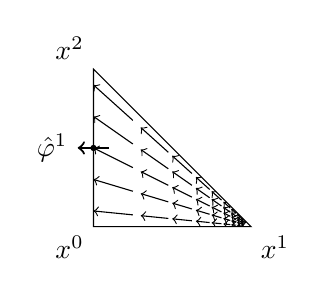
\begin{tikzpicture}[scale=2]
  \begin{scope}
    \draw[clip] (0,0) -- (1,0) -- (0,1) --cycle;
    \foreach \y in {.1,.3,...,.9}
      \foreach \x in {1,.7,.5,.35,.25,.175,.125,.0875,.0625}
        \draw[<-] (1-\x,\y*\x) -- +(\x/4,-\y*\x/4);
  \end{scope}
  \path (0,0) node[below left] {$x^0$}
        (1,0) node[below right] {$x^1$}
        (0,1) node[above left] {$x^2$};
  \draw[->,thick] (.1,.5) -- (-.1,.5) node[left] {$\hat\varphi^1$};
  \fill (0,.5) circle (.02);
\end{tikzpicture}

These elements have the following property:
\begin{equation}
  \varphi^i(x)\cdot n^j=\delta_{ij}\quad\forall x\in\text{face $j$}
\end{equation}
Here $n^j$ is the outer normal unit vector to face $j$ and $\delta_{ij}$ is
the Kronecker delta.  Naturally, transforming the basis should preserve that
property.  This is achieved by the Piola-transformation:
\begin{equation}
  \varphi^i(\mu(\hat x)) = \frac{\hat J_\mu(\hat x)}{|\hat J_\mu(\hat x)|}
    \hat\varphi^i(\hat x)
\end{equation}

\subsubsection{Edge Elements}

Edge elements are used in finite element electro-magnetics.  In the lowest
order, their dofs are associated with edges, i.e.\ sub-entities of dimension
1.  They can be expressed in terms of first order node-based Lagrange finite
elements $L^i$ as follows:
\begin{equation}
  N^i = \ell^i(L^{i_0} \nabla L^{i_1} - L^{i_1} \nabla L^{i_0})
\end{equation}
Here $i_0$ and $i_1$ are the indices of the nodes at the endpoints of edge $i$ and
$\ell^i$ is the length of edge $i$.

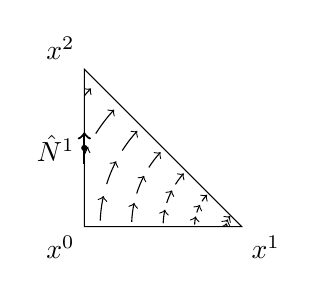
\begin{tikzpicture}[scale=2]
  \begin{scope}
    \draw[clip] (0,0) -- (1,0) -- (0,1) --cycle;
    \foreach \x in {.1,.3,...,1.5}
      \foreach \a in {2.5,17.5,32.5}
        \draw[->] (1,0) +(180-\a:\x) arc(180-\a:170-\a:\x);
  \end{scope}
  \path (0,0) node[below left] {$x^0$}
        (1,0) node[below right] {$x^1$}
        (0,1) node[above left] {$x^2$};
  \draw[->,thick] (0,.4) -- (0,.6);
  \fill (0,.5) circle (.02) node[left] {$\hat N^1$};
\end{tikzpicture}

Edge elements have a similar property as Raviart-Thomas elements: the
tangential component is 1 on the associated edge and 0 on all other edges:
\begin{equation}
  N^i(x)\cdot t^j=\delta_{ij}\quad\forall x\in\text{edge $j$}
\end{equation}

For the transformation we make the ansatz
\begin{equation}
  N^i(\mu(\hat x)) = \alpha^iA\hat N^i(\hat x)
\end{equation}
with the scalars $\alpha^i$ and a matrix $A$.  We express $N^i$ and $\hat N^i$
in terms of the corresponding P1 bases
\begin{equation}
  \ell^i\{L^{i_0}(\mu(\hat x)) \cdot \nabla L^{i_1}|_{\mu(\hat x)}
          - L^{i_1}(\mu(\hat x)) \cdot \nabla L^{i_0}|_{\mu(\hat x)}\}
  = \alpha^iA\hat\ell^i\{
          \hat L^{i_0}(\hat x) \cdot \hat\nabla\hat L^{i_1}|_{\hat x}
        - \hat L^{i_1}(\hat x) \cdot \hat\nabla\hat L^{i_0}|_{\hat x}\}
\end{equation}
By replacing the global P1 bases by the their transformations
\begin{align}
  L^i(\mu(\hat x)) &= \hat L^i(\hat x) \\
  \nabla L^i|_{\mu(\hat x)} &= \hat J_\mu^{-T}(\hat x) \hat\nabla\hat L^i|_{\hat x}
\end{align}
we obtain
\begin{multline}
  \ell^i\hat J_\mu^{-T}(\hat x)\{
          \hat L^{i_0}(\hat x) \cdot \hat\nabla\hat L^{i_1}|_{\hat x}
        - \hat L^{i_1}(\hat x) \cdot \hat\nabla\hat L^{i_0}|_{\hat x}\} \\
  = \alpha^iA\hat\ell^i\{
          \hat L^{i_0}(\hat x) \cdot \hat\nabla\hat L^{i_1}|_{\hat x}
        - \hat L^{i_1}(\hat x) \cdot \hat\nabla\hat L^{i_0}|_{\hat x}\}
\end{multline}
The expression inside the curly braces on both sides is the same.  We identify
\begin{align}
  A &= \hat J_\mu^{-T}(\hat x) \\
  \alpha^i &= \ell^i/\hat\ell^i
\end{align}
The full transformation then looks like this:
\begin{equation}
  N^i(\mu(\hat x)) = \frac{\ell^i}{\hat\ell^i}
    \hat J_\mu^{-T}(\hat x) \cdot \hat N^i(\hat x)
\end{equation}
Note that this transformation only works for the base functions, not for
superpositions of them.  Each base function $N^i$ has a different
transformation because the base multiplier $\alpha^i$ depends on the number of
the base function.

\subsubsection{Conclusions}

From the examples above we can conclude that the following information is
needed from a {\tt Geometry} class.  It is quite possible that the list below
is incomplete since the examples above may have missed some piece of
information that may be needed in general.
\begin{itemize}
\item The inverse transposed of the Jacobian $\hat J_\mu^{-T}(\hat x)$.
\item The Jacobian itself $\hat J_\mu(\hat x)$.
\item The determinant of the Jacobian $|\hat J_\mu(\hat x)|$.
\item The lengths of the edges of the grid element $\ell^i$.
\item The lengths of the edges of the reference element $\hat\ell^i$.
\end{itemize}
When local coordinates $\hat x$ are provided the local-to-global map $\mu(\hat
x)$ and its inverse $\mu^{-1}(x)$ as well as the corner coordinates $x^i$
themselves are never needed.  This makes the required information independent
of a shift in the global coordinates and opens an optimisation possibility for
regular grids.

\subsection{Vertex Ordering}

The vertex ordering information is based completely on the global numbering of
the
vertices of a grid element.  To obtain it, we collect the global IDs of the
vertices in a vector indexed by the indices of the vertices within the
reference element:
\begin{lstlisting}
void collectVertexIds(const Element& e, const GlobalIdSet& idSet,
                      std::vector<GlobaIdSet::IdType>& ids) {
  ids.resize(e.geometry().corners());
  for(int i = 0; i < ids.size(); ++ids)
    ids[i] = idSet.subId(e, i, Element::dimension);
}
\end{lstlisting}
In the next step the {\em ordering reduction} operation is applied: the
smallest id in the array is replaced by the number 0, the second-smallest is
replaced by the number 1 etc.
\begin{lstlisting}
template<class InIterator, class OutIterator>
void reduceOrder(const InIterator& inBegin, const InIterator& inEnd,
                 OutIterator outIt)
{
  static const std::less<
    typename std::iterator_traits<InIterator>::value_type
    > less;

  for(InIterator inIt = inBegin; inIt != inEnd; ++inIt, ++outIt)
    *outIt = std::count(inBegin, inEnd, std::bind2nd(less, *inIt));
}
\end{lstlisting}
To obtain an actual vector of reduced indices one can use the following code:
\begin{lstlisting}
std::vector<typename GlobalIdSet::IdType> ids;
collectVertexIds(elem, globalIdSet, ids);
std::vector<std::size_t> reduced_indices(ids.size());
reduceOrder(ids.begin(), ids.end(), reduced_indices.begin());
\end{lstlisting}

As an example, lets assume we have a quadrilateral or a tetrahedron with the
global ids of the vertices being 14 for vertex 0, 27 for vertex 1, 3 for
vertex 2 and 800 for vertex 3.  After ordering reduction the reduced vector
will contain 1, 2, 0 and 3 in that order.

When determining the vertex ordering for a sub-entity, the reduced indices
corresponding to the vertices sub-entity are extracted into a smaller vector
and the reduction is applied again, at least conceptually.  In reality, the
reduction is mostly only necessary because the type of the global ids may be a
complicated non-integral struct, and we want to keep the vertex ordering
information as lean as possible.  The actual information is always contained
in the relative
ordering of the indices/ids, and the reduction preserves that.

The ordering information can always be obtained from the global ids of the
vertices.  However, for some grids, such as ALUGrid, using the global ids is
quiet expensive.  On the other hand, ALUGrid already stores a twist of the
faces, which can be easily extracted and contains the same information as the
vertex ordering, just encoded in a different way.  Though this does not
provide vertex ordering information for the whole element, this information is
seldom needed.

To accommodate all sides, we define an interface class {\tt
  VertexOrderingInterface}.  Implementations of this interface can be used to
provide vertex ordering information.  Grids that store the vertex ordering
internally for certain sub-entities can provide an optimised implementation.
These implementations may omit vertex ordering information for sub-entities
where such information is not readily available; they should throw {\tt
  NotImplemented} if such information is requested anyway.

Note that the information is still required to be consistent for those
sub-entities where information is available: Consider a tetrahedron and pick
two triangular faces $A$ and $B$ with a common edge.  If someone requests
vertex ordering information for one of the faces and reduces that information
to the edge, the result must be the same no matter whether face $A$ or $B$ was
used or whether the ordering was requested directly for the edge itself.

The interface for the class is as follows:
\begin{lstlisting}
struct VertexOrderingInterface {
  // dimension of the entity this applies to
  static const std::size_t dimension;
  // geometry type of the entity this applies to
  const GeometryType type() const;

  // iterate over some sub-entity's vertex indices
  // must be a RandomAccess iterator, value_type may be constant
  class iterator;

  // get begin iterator for the vertex indices of some sub-entity
  iterator begin(std::size_t codim, std::size_t subEntity) const;
  // get end iterator for the vertex indices of some sub-entity
  iterator begin(std::size_t codim, std::size_t subEntity) const;

  // get reduced vertex ordering for the specified sub-entity
  void getReduced(std::size_t codim, std::size_t subEntity,
                  std::vector<std::size_t>& order) const;
};
\end{lstlisting}
Information about the dimension and the geometry type is included because it
determines the limits for the parameters (via the {\tt
  GenericReferenceElements}).  The {\tt getReduced()} method shall resize the
vector passed in the {\tt order} parameter to the suitable size.

\subsection{Matching Multiple Dofs on a Common Sub-Entity}

Some finite elements have more than one dof on a given sub-entity of an
element, and assign a position inside the sub-entity to that dof (i.e.\ Pk
$k\geq4$, Qk $k\geq3$).  For conforming schemes the ordering of the dofs on a
sub-entity shared by two or more elements must match such that the dofs on the
same position can be identified.

A similar situation arises with edge elements of order $1.5$: For simplices
they have three base functions on a face but only two of them are independent.
A finite element implementation must make sure to pick the same two base
functions for the face in neighbouring elements so their dofs can be
identified.

Both issues can be addressed using the information provided by the ordering of
the global ids of the vertices.

\subsection{Flipping of Base Function Values}

Some finite element families, most notably Raviart-Thomas and edge elements,
assign an orientation to (some of) their dofs.  That is, the value of the dof
$a^i$ is interpolated from a function $u$ as the functions value at the dofs
position $x^i$ projected onto some unit vector $e^i$:
\begin{equation}
  a^i = u(x^i)\cdot e^i
\end{equation}
The direction of that unit vector is the orientation of the dof.  For
Raviart-Thomas $e^i$ is the unit vector normal to the face (codimension 1
sub-entity), for edge elements $e^i$ is the unit vector tangential to the edge
(dimension 1 sub-entity) on which the dof is located.

To be continuous over element borders, elements connected to a common
sub-entity must agree upon a common global orientation for that sub-entity.
If their local orientation differs from the global orientation, the {\tt
  GlobalValueBasis} must multiply the value of the corresponding basis
function by $-1$.  The tricky part is the to determine the global orientation
for the common sub-entity correctly.

\subsubsection{Tangential Orientation for Lines}

Lines have two vertices which can be used to choose the orientation of the
line: the orientation vector points from the vertex with the lower index/id to
the vertex with the higher index/id.  That is the geometric interpretation, we
actually don't want to compare coordinates, but preferably just integers.

To obtain the local orientation, of an edge in an element, collect the
indices of the edges vertices, and here we mean {\em indices inside the
  reference element} of the element:
\begin{lstlisting}
unsigned local_orientation[2];
local_orientation[0] = refelem.subEntity(edge_index, dim-1, 0, dim);
local_orientation[1] = refelem.subEntity(edge_index, dim-1, 1, dim);
\end{lstlisting}

For the global orientation we do basically the same.  However, this time we
use the vertex ordering information derived from the global ids of the
vertices of
the element instead of vertex indices inside the reference element:
\begin{lstlisting}
unsigned global_orientation[2];
global_orientation[0] = vertex_order[local_orientation[0]];
global_orientation[1] = vertex_order[local_orientation[1]];
\end{lstlisting}

The ordering of the index values determines the local and global orientation:
\begin{lstlisting}
if((local_orientation[0] < local_orientation[1])
   == (global_orientation[0] < global_orientation[1]))
{
  // local and global orientation are identical; nothing to do
} else {
  // local and global orientation differ; flip base function value
}
\end{lstlisting}

\subsubsection{Normal Orientation for Codimension 1 Sub-Entities}

Normal orientation for sub-entities of codimension 1 is important for
Raviart-Thomas elements.  Normal orientation is more tricky and cannot be done
using the ordering of the indices/id of the corners alone.  Some additional
information is needed, such as the sign of the determinant of the Jacobian of
the geometry map $\sgn(\det(\hat J_\mu))$.  This is however not enough for
lower dimensional grids in a higher dimensional world, since then the Jacobian
is no longer quadratic and has no determinant.

The reason why the information about the vertex ids is not enough is roughly
that to construct the normal orientation there is alway some kind of rotation
involved.  In 2D the codimension 1 sub-entities are edges.  We can obtain a
normal orientation by rotating the tangential orientation by $90�$.  To get a
consistent result however, this rotation must be done in the global coordinate
system for the global orientation and in the respective local coordinate
systems for the local orientations.  Locally on the element we have only the
local coordinate system available, however.  If the geometric transformation
$\mu$ involves mirroring, then the sense of the rotation will be different for
the local and the global coordinate system.  The sign of the Jacobian's
determinant can tell us whether there is mirroring involved or not.

In 3D the construction of the orientation differs: for triangles we walk
through the indices/ids in ascending order and determine the direction of the
normal vector by the right-hand rule:
\\\hspace*{\fill}
  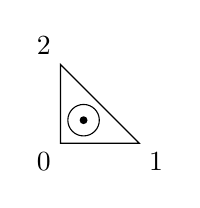
\begin{tikzpicture}
    \draw (0,0) node[below left] {0}
       -- (1,0) node[below right] {1}
       -- (0,1) node[above left] {2}
       --cycle;
    \coordinate (c) at (.29289,.29289);
    \draw (c) circle (.2);
    \fill (c) circle (.05);
  \end{tikzpicture}
  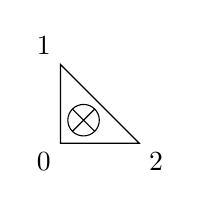
\begin{tikzpicture}
    \draw (0,0) node[below left] {0}
       -- (1,0) node[below right] {2}
       -- (0,1) node[above left] {1}
       --cycle;
    \coordinate (c) at (.29289,.29289);
    \draw (c) circle (.2);
    \draw (c) +(45:.2) -- +(45:-.2)
              +(-45:.2) -- +(-45:-.2);
  \end{tikzpicture}
\hspace*{\fill}\\
Similar for quadrilaterals, although if their indices/ids are acyclic we just
have to pick and orientation (here we chose to ignore the highest index/id and
determine the orientation from the remaining indices/ids as for triangles):
\\\hspace*{\fill}
  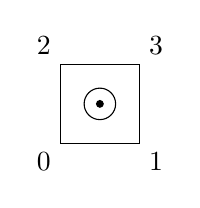
\begin{tikzpicture}
    \draw (0,0) node[below left] {0}
       -- (1,0) node[below right] {1}
       -- (1,1) node[above right] {3}
       -- (0,1) node[above left] {2}
       --cycle;
    \coordinate (c) at (.5,.5);
    \draw (c) circle (.2);
    \fill (c) circle (.05);
  \end{tikzpicture}
  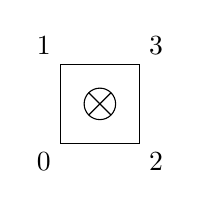
\begin{tikzpicture}
    \draw (0,0) node[below left] {0}
       -- (1,0) node[below right] {2}
       -- (1,1) node[above right] {3}
       -- (0,1) node[above left] {1}
       --cycle;
    \coordinate (c) at (.5,.5);
    \draw (c) circle (.2);
    \draw (c) +(45:.2) -- +(45:-.2)
              +(-45:.2) -- +(-45:-.2);
  \end{tikzpicture}
  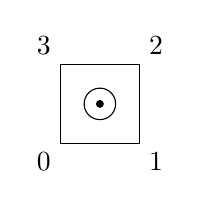
\begin{tikzpicture}
    \draw (0,0) node[below left] {0}
       -- (1,0) node[below right] {1}
       -- (1,1) node[above right] {2}
       -- (0,1) node[above left] {3}
       --cycle;
    \coordinate (c) at (.5,.5);
    \draw (c) circle (.2);
    \fill (c) circle (.05);
  \end{tikzpicture}
  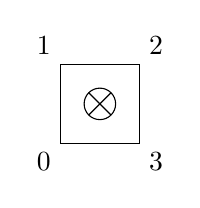
\begin{tikzpicture}
    \draw (0,0) node[below left] {0}
       -- (1,0) node[below right] {3}
       -- (1,1) node[above right] {2}
       -- (0,1) node[above left] {1}
       --cycle;
    \coordinate (c) at (.5,.5);
    \draw (c) circle (.2);
    \draw (c) +(45:.2) -- +(45:-.2)
              +(-45:.2) -- +(-45:-.2);
  \end{tikzpicture}
\hspace*{\fill}

This is all rather tedious and in fact there is a much simpler way, which will
even work in the case of lower-dimensional grids in a higher-dimensional
world.  Sub-entities of codimension 1 are always situated between two
Elements.  Choosing a normal orientation for the sub-entity means to choose a
vector that points from one element into the other.  The global orientation
can thus be chosen by comparing the ids of the elements: it points outward in
the element with the lower id and inward in the element with the higher id.

The face orientation should be passed as a bool vector:
\begin{lstlisting}
typedef std::vector<bool> FaceOrientation;
\end{lstlisting}
The vector is indexed by the index of the face in the reference element.  A
value of {\tt true} means the global orientation of the face is outward, {\tt
  false} means it is inward.

\subsection{API}

The API for global-valued finite elements consists of five interface classes
({\tt Global\-Value\-Basis\-Interface}, {\tt
  GlobalValueInterpolationInterface}, {\tt
  Global\-Value\-Coefficients\-Interface}, {\tt
  GlobalValueFiniteElementInterface}, and {\tt
  Global\-Value\-Finite\-Element\-Factory\-Interface}) and two traits classes
({\tt GlobalValueBasisTraits} and {\tt
  Global\-Value\-Finite\-Element\-Traits}).  The name prefix ``{\tt
  GlobalValue}'' was chosen because these finite elements deal with global
base function values, but still take local coordinates on the reference
element.

\subsubsection{Finite Element Interface}

\begin{lstlisting}[escapechar=\$]
struct GlobalValueFiniteElementInterface
{
  // types of component objects
  struct Traits
  {
    typedef $\em implementation-defined$ Basis;
    typedef $\em implementation-defined$ Coefficients;
    typedef $\em implementation-defined$ Interpolation;
  };

  // constructor arguments a implementation specific
  GlobalValueFiniteElementInterface(...);
  // ... except for the copy constructor
  GlobalValueFiniteElementInterface
    (const GlobalValueFiniteElementInterface&);

  // extract component objects
  const typename Traits::Basis& basis() const;
  const typename Traits::Coefficients& coefficients() const;
  const typename Traits::Interpolation& interpolation() const;
  GeometryType type() const;
};
\end{lstlisting}
The member class {\tt Traits} may be a member typedef instead.  Constructor
signatures and existence is implementation-defined, except for the copy
constructor, which must be present and publicly accessible.  Construction is
generally done by a factory class.  To keep copy-construction efficient it is
recommended that instances of this class are light proxy objects.

The reason to mandate copy-construction is as follows: Up to now with local
finite elements \modulename{dune-pdelab} used the class {\tt FiniteElementMap}
as a kind of finite element factory.  If the finite element was required in
different variants for a given grid (i.e.\ because normal continuity was
required for Raviar-Thomas elements), the {\tt FiniteElementMap} would store
all the variants internally and return a reference to the correct variant upon
request.  Since global-valued finite elements depend on the geometry of the
grid element, this trick is no longer useful, especially if you plan to modify
the finite element object by ``binding'' it to the geometry.  The problem is
that more than one finite element for different grid elements may be required
at the same time (think iterating over the intersections).  If the {\tt
  FiniteElementMap} returns the same variant for both grid elements the user
code will first bind the finite element to the inside element and later to the
outside element, since both of his finite element references point to the same
object.  Thus when he tries to access the inside finite element, he will in
reality access the outside element.

\subsubsection{Finite Element Factory Interface}

\begin{lstlisting}[escapechar=\$]
template<class Geometry>
struct GlobalValueFiniteElementFactoryInterface
{
  // may also be an inline class
  typedef $\em implementation-defined$ FiniteElement;

  // construction is implementation-defined
  GlobalValueFiniteElementFactoryInterface(...);

  // finite element object creation
  // arguments are implementation defined
  const FiniteElement make(...);
};
\end{lstlisting}
The method to create a finite element object is {\tt make()}.  The created
object is returned by value ({\tt const FiniteElement}).  The factory
implementation may choose to return by reference instead ({\tt const
  FiniteElement\&}).  Because temporaries may be bound to const references in
C++, this way code using the factory can always bind the returned value to a
const reference and avoid copy construction if that is not necessary:
\begin{lstlisting}
const Factory::FiniteElement& fe = factory.make();
\end{lstlisting}
In any case, the returned value or reference must be valid for as long as the
factory object exists.

Since each finite element family will need different information to create a
finite element object tailored to a particular grid element, the actual
argument of the {\tt male()} are implementation-defined.  Earlier in this
section we have seen different types of information which may be needed to
create a tailored finite element: geometry, vertex ordering and face
orientation.
If they are needed for a given finite element implementation, that finite
element should require necessary items in the order given above and in the
encoding given earlier.  If neither geometry nor vertex ordering is required,
but the geometry type is, that should be given in place of geometry and vertex
ordering
directly.  Any extra information should be given after these arguments.  The
possible signatures for make thus are:
\begin{lstlisting}
make(const Geometry&, const VertexOrder&, const FaceOrientation&, ...);
make(const Geometry&, const VertexOrder&, ...);
make(const Geometry&, const FaceOrientation&, ...);
make(const Geometry&, ...);
make(const VertexOrder&, const FaceOrientation&, ...);
make(const VertexOrder&, ...);
make(const GeometryType&, const FaceOrientation&, ...);
make(const GeometryType&, ...);
make(const FaceOrientation&, ...);
make(...);
\end{lstlisting}
Implementation must document what kind of arguments are required for {\tt
  make()}.

The constructor signature is implementation-defined.

It is recommended that the factory caches as much information as possible.
For instance, for regular hypercube grids the Jacobian of the geometry does
not change and is the only thing needed to transform the derivatives.  For
this case the constructor should take a sample geometry and precompute the
transformation.  Whether the regular and the general case are distinguished by
different constructor arguments to the same factory class, or whether there is
one factory class for the regular and one for the general case is left to the
implementor of the factory.

\subsubsection{Basis Interface}
\begin{lstlisting}[escapechar=\$]
struct GlobalValueBasisInterface
{
  struct Traits
  {
    // domain properties (local and global)
    typedef $\em implementation-defined$ DomainField;
    static const std::size_t dimDomainLocal = $\em implementation-defined$;
    static const std::size_t dimDomainGlobal = $\em implementation-defined$;
    typedef $\em implementation-defined$ DomainLocal;
    typedef $\em implementation-defined$ DomainGlobal;

    // range properties (global range only)
    typedef $\em implementation-defined$ RangeField;
    static const std::size_t dimRange = $\em implementation-defined$;
    typedef $\em implementation-defined$ Range;

    // jacobian properties (dimRange x dimDomainGlobal Matrix with
    // components of type RangeField)
    typedef $\em implementation-defined$ Jacobian;

    // maximum number of partial derivatives supported
    static const std::size_t diffOrder = $\em implementation-defined$;
  };

  // Number of shape functions
  std::size_t size () const;
  // Polynomial order of the shape functions for quadrature
  std::size_t order () const;

  // Evaluate all shape functions at given position
  void evaluateFunction
  ( const typename Traits::LocalDomain& in,
    std::vector<typename Traits::Range>& out) const;

  // Evaluate jacobian of all shape functions at given position
  // required for Traits::diffOrder >= 1
  void evaluateJacobian
  ( const typename Traits::LocalDomain& in,
    std::vector<typename Traits::Jacobian>& out) const;

  // Evaluate derivatives of all shape functions at given position
  // required for Traits::diffOrder >= 2
  void evaluate
  ( const array<std::size_t,Traits::dimGlobalDomain>& directions,
    const typename Traits::LocalDomain& in,
    std::vector<typename Traits::Range>& out) const;
};
\end{lstlisting}
The basis interface closely follows the local basis interface with some
notable exceptions.

First there are the types in the traits class.  Since coordinates are still given
in the reference elements coordinate system but derivatives are done with
respect to global coordinates, a distinction must be made between local and
global domain.  The other change is that the member types of the traits class
no longer have a suffix ``{\tt Type}'' since it is quite clear from the
camel-case naming convention that they are types.

Second the method for general derivatives {\tt evaluate()} is no longer a
template method and its argument {\tt directions} has different semantics.  In
the local basis interface, {\tt directions} was a list of directions in which
to take derivatives, i.e.\ {\tt directions=\{0, 1, 0, 2\}} for the derivative
$\partial_0\partial_1\partial_0\partial_2$.  This is inconvenient since it
requires {\tt directions} to be a list of variable length, making the length a
template parameter, and because the order implied in the above derivative does
not really exist, it can just as well be written as
$\partial_0^2\partial_1\partial_2$.  So in the global-value interface {\tt
  directions} lists the exponents in the last expression: {\tt direction=\{2,
  1, 1\}}.  This way the length of {\tt directions} will always be {\tt
  Traits::dimDomainGlobal} and {\tt evaluate()} no longer needs to be a
template.

\subsubsection{Interpolation Interface}

\begin{lstlisting}
struct GlobalValueInterpolationInterface
{
  // Export basis traits
  typedef GlobalValueBasisInterface::Traits Traits;

  // determine coefficients interpolating a given function
  template<typename F, typename C>
  void interpolate (const F& f, std::vector<C>& out) const;
};
\end{lstlisting}
The interface for global-value interpolation objects also has little
modifications compared to local interpolation objects.  Main addition is the
member type {\tt Traits} which is the same as in the corresponding basis
class.  This is to document the parameter types that {\tt interpolate()} will
use to evaluate the function {\tt f}.

For the member method {\tt evaluate()} the requirements for the function
object {\tt f} change slightly: it is still required to support the expression
{\tt f.evaluate(x, y)}, and {\tt x} in that expression is still a local
coordinate (though the type is named a little bit different: {\tt const
  Traits::DomainLocal\&}.  The difference is that the returned value {\tt y}
is now in global coordinates and of the type {\tt Traits::Range}.

\subsection{Coefficients Interface}

\begin{lstlisting}
struct GlobalValueCoefficientsInterface
{
  // number of coefficients
  std::size_t size() const;

  // get i'th index
  const LocalKey& localKey(std::size_t i) const;
};
\end{lstlisting}
The interface for the coefficients class is exactly the same as for the local
coefficients.  If the global-valued finite elements is implemented in term of
a local finite element it will often be possible to simply reuse the
coefficients class of the local finite element.

If there is some dof-matching required for common sub-entities of neighbouring
elements however, and this dof-matching can be done entirely by reordering the
dofs on the sub-entity, then the coefficients class is the place to do it.

\section{Appendix: List of Available Elements}



% bibtex bibliography
%\bibliographystyle{plain}
%\bibliography{istl.bib}


\end{document}
